\chapter{Introduction}\label{chap:introduction}
\graphicspath{{Chapter1/}}

\section{Background}
	Recent decade has witnessed a growing interest in Artificial Intelligence (AI), big data, and High-performance Computing (HPC). The digitalization infrastructure produces a large amount of data, significantly advancing the state-of-the-art of AI. Meanwhile, the fast pace of developing computing facilities enables the learning-based optimization models to learn from large-scale big data efficiently. Assisted by strong computational power and big data, deep learning technologies have reformulated and empowered a wide variety of applications in business, industry, and academia~\citep{lecun2015deep, bommasani2021opportunities}. The incredibly powerful learning and generalization capability of deep learning encourages us to embrace emergent and novel technologies to address fundamental, critical, and urgent problems in this day and age, such as drug discovery for the treatment of COVID-19 and cancer, health promotion and disease prevention, climate change, natural disasters forecasting, protein structure prediction, nuclear fusion control, and Artificial General Intelligence (AGI). In addition, the homogenization of deep learning models has been established and verified by different disciplines,~\eg, physics, chemistry, biology, computational neuroscience, medicine, mathematics, and computer science. Nowadays, deep learning algorithms have gradually become one of the~\textit{de~facto} standards. Powered by them, AI and big data are making a vast difference in society. They are directing to the next industrial revolution,~\ie, the intelligence revolution, which would dramatically transform business and industry, significantly promote productivity, and widely benefit humanity.
	
	Recently, Computer Vision (CV) has gained much more popularities with the construction of large-scale visual databases,~\eg, ImageNet~\citep{deng2009imagenet}, and the usage of extremely powerful computational devices, such as NVIDIA Graphics Processing Unit (GPU) clusters and Google Tensor Processing Unit (TPU) pods. Tasting the values of emergence and homogenization properties of deep learning, models' performance has been remarkably improved across tasks, such as image and video analytics, 3D vision processing, natural language processing, automatic speech recognition, and recommendation systems. 
	
	Among deep learning algorithms, Convolutional Neural Network (CNN) is insanely effective and efficient, and the ``unreasonable" effectiveness of deep feature representation has triggered much attention from researchers and engineers in academia and industry~\citep{lecun1998gradient, zhang2018unreasonable, SimonyanZ14a, ding2021comparison, dingIQA}. By learning from large-scale visual data, CV algorithms are capable of understanding the content and context of images and videos. Such semantics and content understanding for relational and dependency modeling is one of the keys to successful modern CV systems.
	
	\subsection{Visual Quality Assessment}
	Over decades, visual quality assessment has been one of the most fundamental, essential, and indispensable CV tasks by virtue of its functionalities, such as quality assessment, performance evaluation, and parameter optimization~\citep{ding2021comparison}. It is applied to a wide variety of mediums, such as images, videos, point clouds, and mesh. Among them, images and videos play an increasingly influential position in our daily life because they are one of the immediate communication mediums among people. Hereby, we take images and videos as an example. First of all, visual quality assessment methods measure the input images/videos' quality, which is one of the fundamental attributes of images/videos. Secondly, by estimating the visual quality of the predicted or generated images/videos, we can evaluate the performances of different image/video processing systems,~\eg, effectiveness, robustness, generalization capability, optimization capability, discriminability, transferability, and efficiency. Making use of visual quality assessment, advanced methods can be explored for specific applications, such as underwater image enhancement and restoration~\citep{GuoTMM}. Lastly, various image processing systems can be optimized via an image quality assessment metric. For example, an image restoration method can be optimized end-to-end via a perceptually relevant image fidelity metric as the loss function, replacing the Mean Squared Error (MSE) or~$\mathrm{L_1}$~Loss~\citep{ding2021comparison}. Another example is that some parameters of an image processing algorithm,~\eg, noise variance, can be estimated by a quality assessment method. Taking benefit of such a method, the optimal parameters can be estimated, and superior performances can be achieved~\citep{mittal2012no, zhu2010automatic}. Thus, the research on visual quality assessment is of great importance in real-world applications.
	
	Besides, visual quality assessment also plays an essential role in streaming media companies, such as Alphabet YouTube, Meta Instagram and Facebook, Hulu, ByteDance TikTok, Baidu iQIYI, Tencent Video, and Netflix. Delivering and generating visually pleasing, human-centric, and high-quality content to customers has become a key competition among tech giants. Visual quality assessment, thus, is indispensable in improving customers' visual experience and optimizing the production line.~\textit{De~facto}, there is a long process for people to perceive images and videos, including image and video acquisition, compression, transmission, restoration, enhancement, and display. While performing any of these steps, images and videos may be distorted, affecting their final display's visual/perceptual quality. The definition of ``visual quality'' refers to people's overall subjective visual experience when viewing and perceiving images and videos. Various factors, such as brightness, contrast, sharpness, color, noise, and compression loss, usually influence visual experience. In this thesis, we pay attention to Image Quality Assessment (IQA). IQA can be categorized into subjective IQA, where image quality is derived from human subjects through subjective experiments, and objective IQA, where image quality is automatically predicted by machines.
	
	\subsection{Subjective Image Quality Assessment}
	Image quality collected from human subjects (observers) is much more accurate, reliable, and trustworthy because it correlates well with human visual perception. There are two broadly used schemes to conduct subjective IQA,~\ie, Single Stimulus (SS) and Pair Comparison (PC). As for the SS method, the subject will be instructed to view one image and assign an absolute quality score. On the other hand, the PC method requests the subject to compare the quality of two images and select which image has the better visual quality. To be more specific, there are six subjective IQA methods, as defined in the Recommendation ITU-R BT.500-14~\citep{bt2020methodologies},~\ie, SS, Stimulus Comparison (SC), Double Stimulus Impairment Scale (DSIS), Double Stimulus Continuous Quality Scale (DSCQS), Subjective Assessment of Multimedia Video Quality (SAMVIQ), and Expert Viewing Protocol (EVP). The PC subjective IQA methods include SC, DSIS, and DSCQS.
	
	\paragraph{SS} To perform SS experiments, the subject will be instructed to view only one image as a single stimulus. The evaluated image would be the reference image and will be randomly displayed.
	
	\paragraph{SC} In the SC method, the subject will be invited to view two images and required to assign a score to represent the relationship between them, such as the visual quality discrepancy.
	
	\paragraph{DSIS} To apply the DSIS method, the subject will be asked to observe the reference image and then view the distorted image. Furthermore, the subject is required to compare the quality between the reference image and the distorted image and assign a quality score for the distorted one. For this method, the suggested experimental duration is within half an hour.
	
	\paragraph{DSCQS} As for the DSCQS method, the subject is instructed to evaluate two images' quality simultaneously.
	
	\paragraph{SAMVIQ} In the SAMVIQ method, the subjects will be asked to evaluate all the distorted images of one reference image at once.
	
	\paragraph{EVP} As for the EVP method, specialists will be recruited and requested to evaluate image quality to reduce the number of subjects.
	
	However, collecting subjective opinions is cumbersome, time-consuming, and expensive. In addition, it cannot be employed to optimize model parameters in image processing systems. As a consequence, subjective studies in data-intensive real-world applications are unrealistic and impractical, and it is crucial to design accurate and efficient objective methods to automatically evaluate image quality. In order to advance objective IQA research, many benchmark databases are constructed to evaluate objective IQA models' performance,~\eg, their effectiveness, robustness, generalization capability, optimization capability, discriminability, transferability, and efficiency. In practice, subjective experiments are mainly conducted under this circumstance. 
	
	In~\reffig{Databases}, we demonstrate some natural images and one screen content image from four IQA benchmark databases (LIVE~\citep{livedataset}, CSIQ~\citep{larson2010most}, TID2013~\citep{ponomarenko2015image}, and KADID-10k~\citep{kadid10k}). In~\reffig{Databases}~(c), the first selected image is a screen content image, and others are natural images. In~\reffig{Databases}~(a),~\reffig{Databases}~(b), and~\reffig{Databases}~(d), all the images are natural images. There are generally three steps to build such a database. First, images are collected and carefully picked to cover a wide variety of content and distortions, as required by specific applications. Second, the recruited subjects are instructed to evaluate the image quality. Lastly, the subjective quality scores are analyzed and post-processed by removing the unqualified subjects and abnormal quality scores. So, image quality is obtained, reflecting the visual experience of the image. In practice, there are two ways to quantify image quality. One way is to use the Mean Opinion Score (MOS) for each image, which is the normalized quality score of all the scores obtained from observers. The other way is to compute the normalized difference of the MOSs between the reference image and the distorted image, namely, the Difference of MOSs Between the Reference and the Distorted Images (DMOS).
	\begin{figure}[!h]
		\centering
		\begin{minipage}[t]{.49\linewidth}
			\centering
			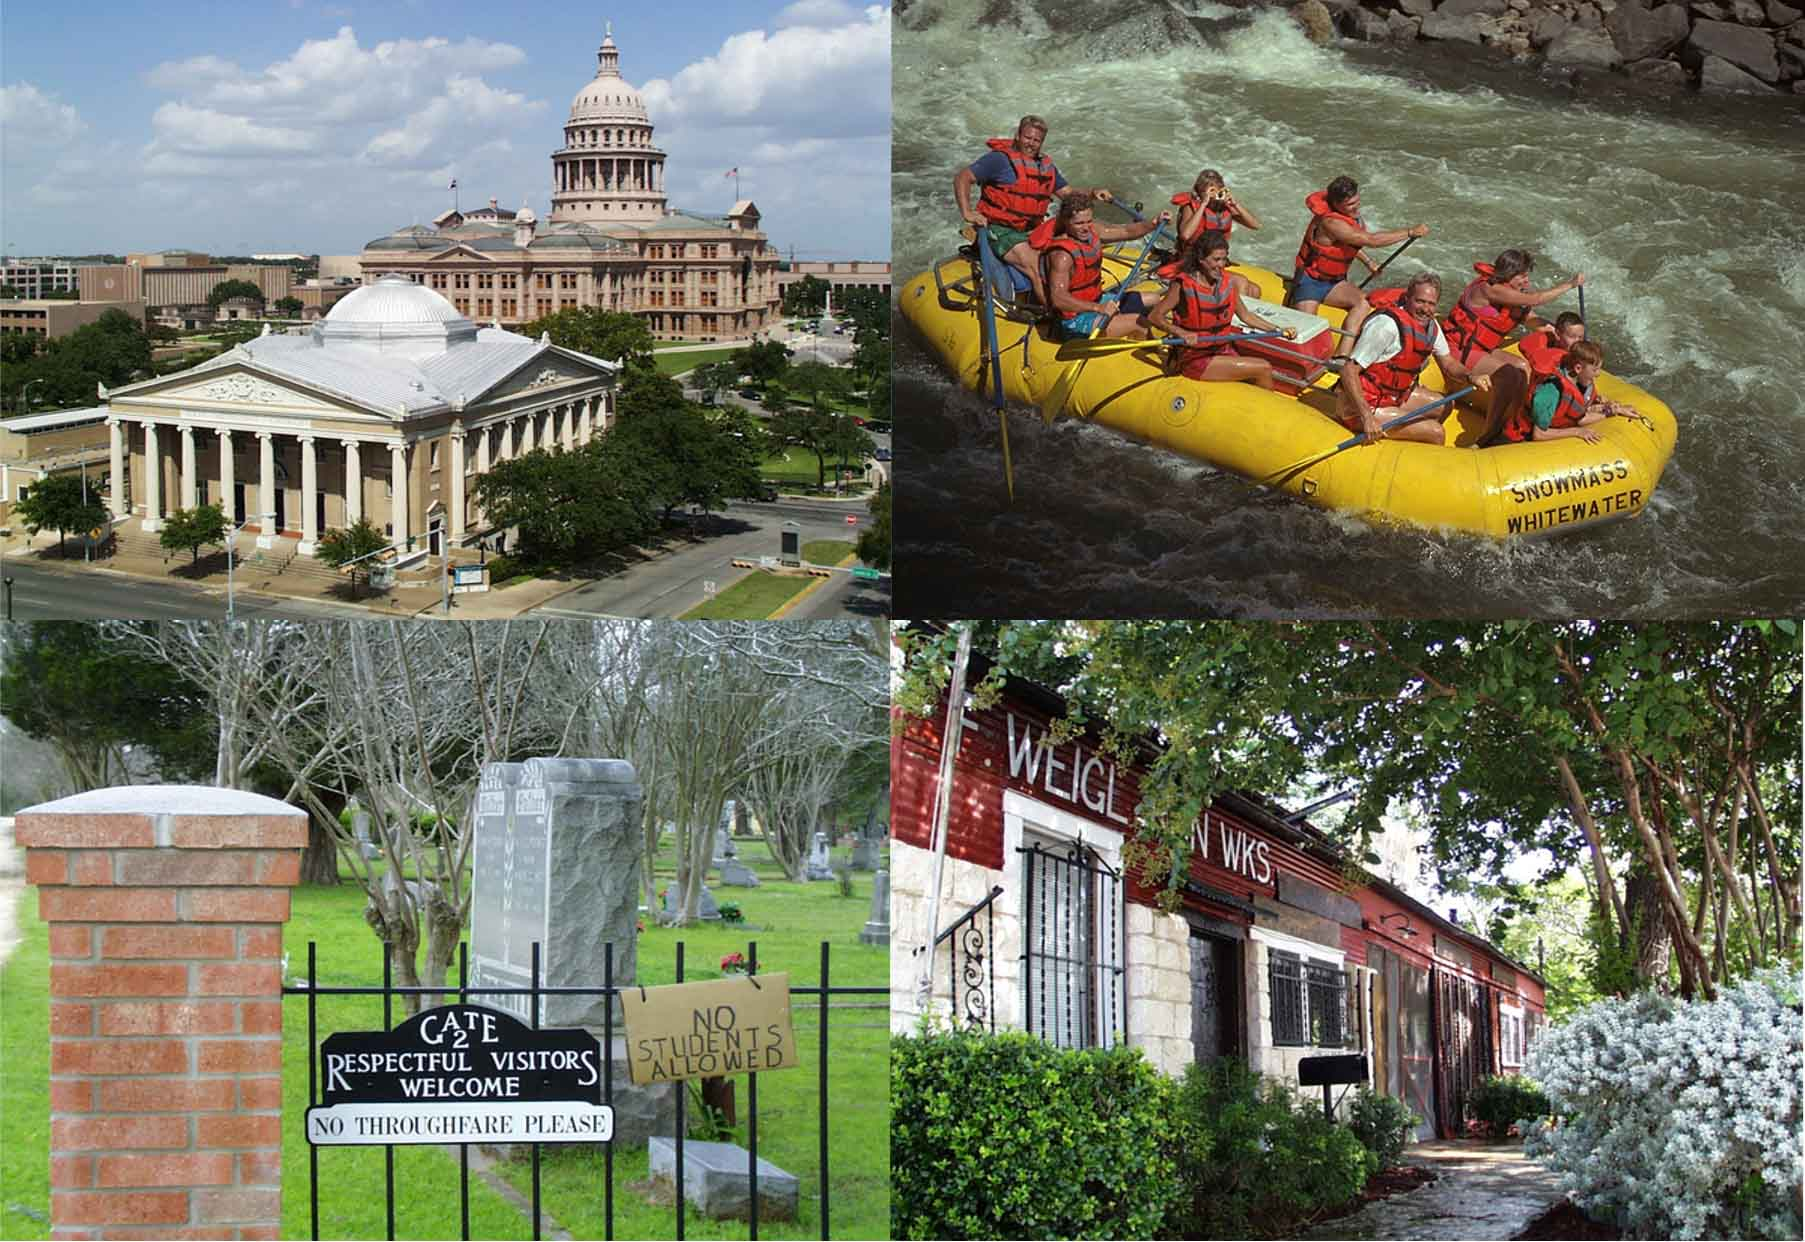
\includegraphics[width=2.8in]{fig/LIVE.jpg}
			\centerline{(a)}
		\end{minipage}
		\begin{minipage}[t]{.49\linewidth}
			\centering
			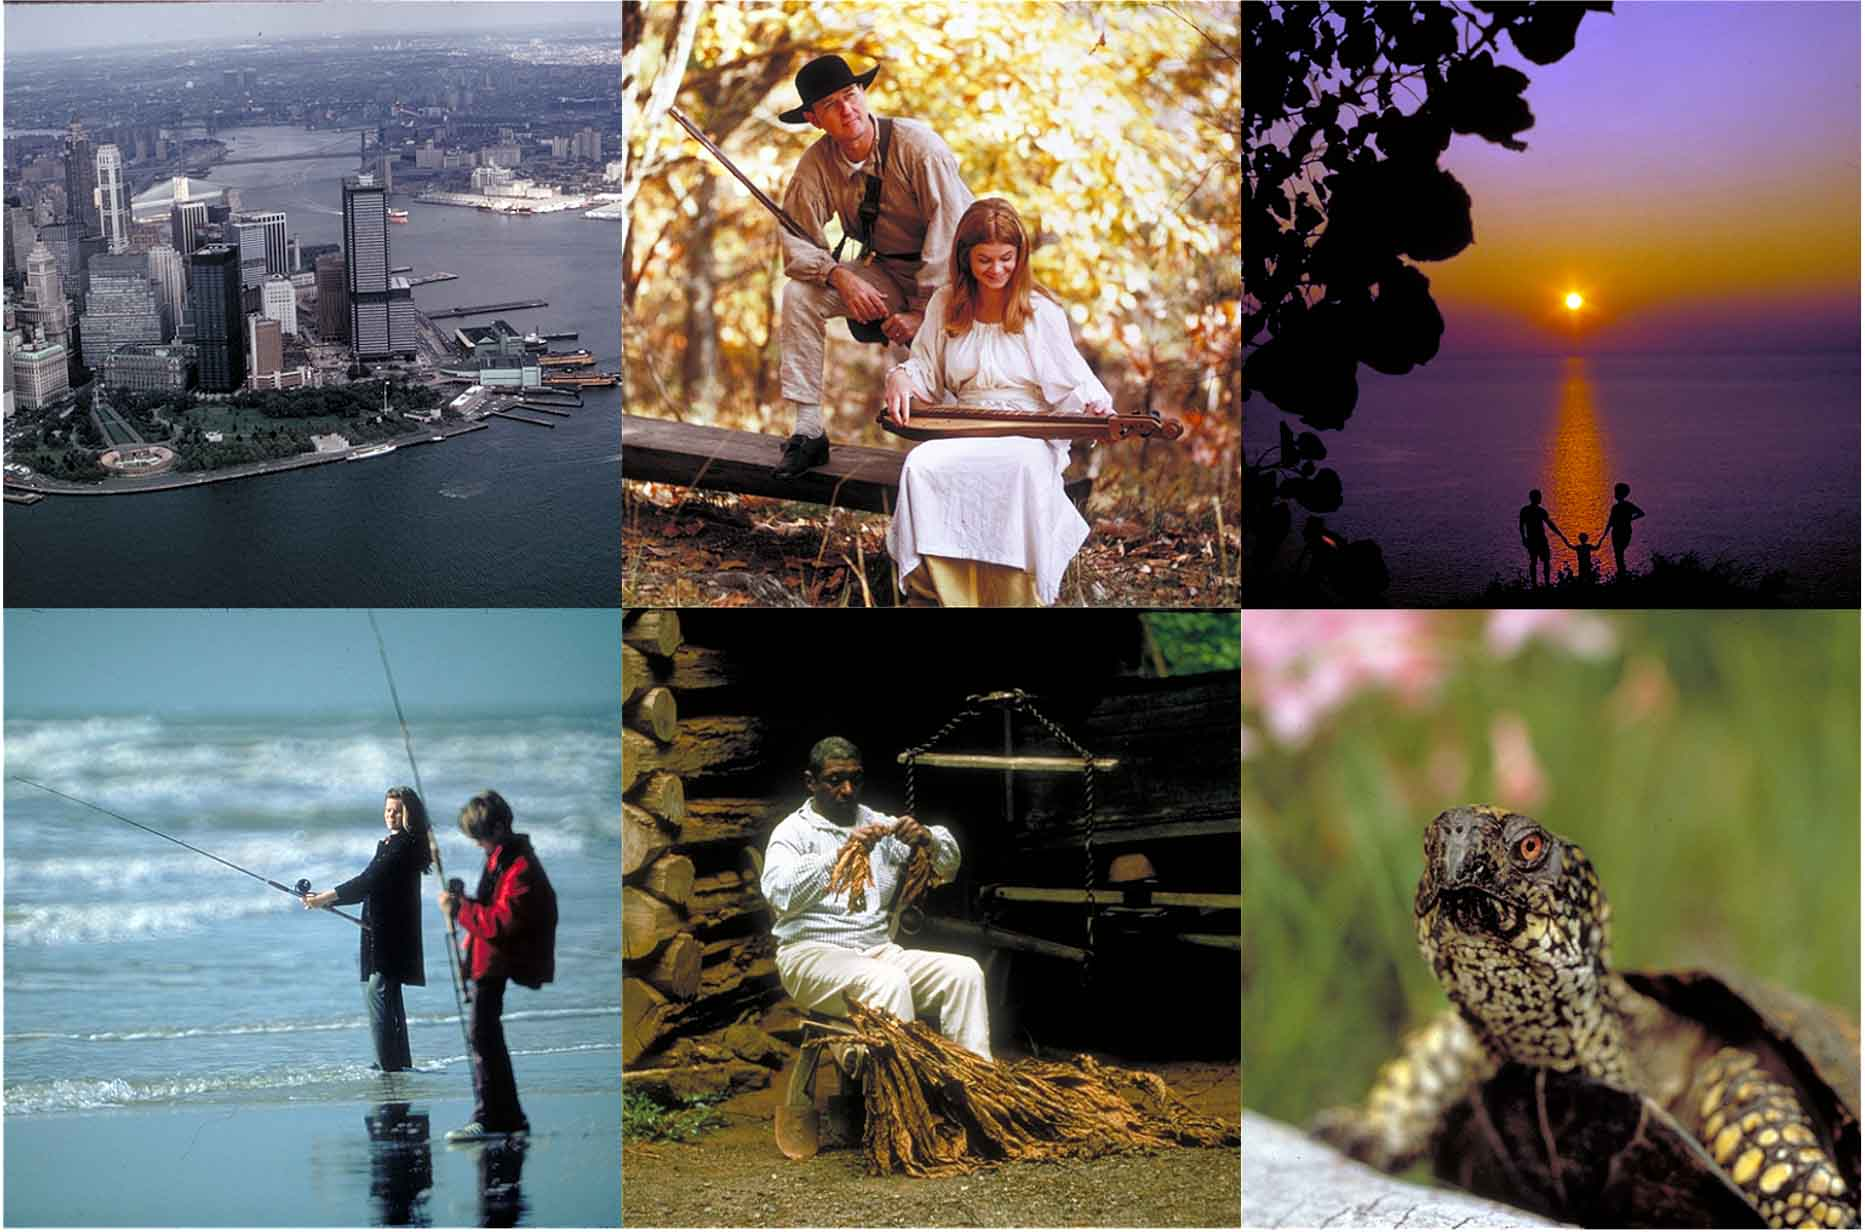
\includegraphics[width=3in, height=1.93in]{fig/CSIQ.jpg}
			\centerline{(b)}
		\end{minipage}
		\begin{minipage}[t]{.49\linewidth}
			\centering
			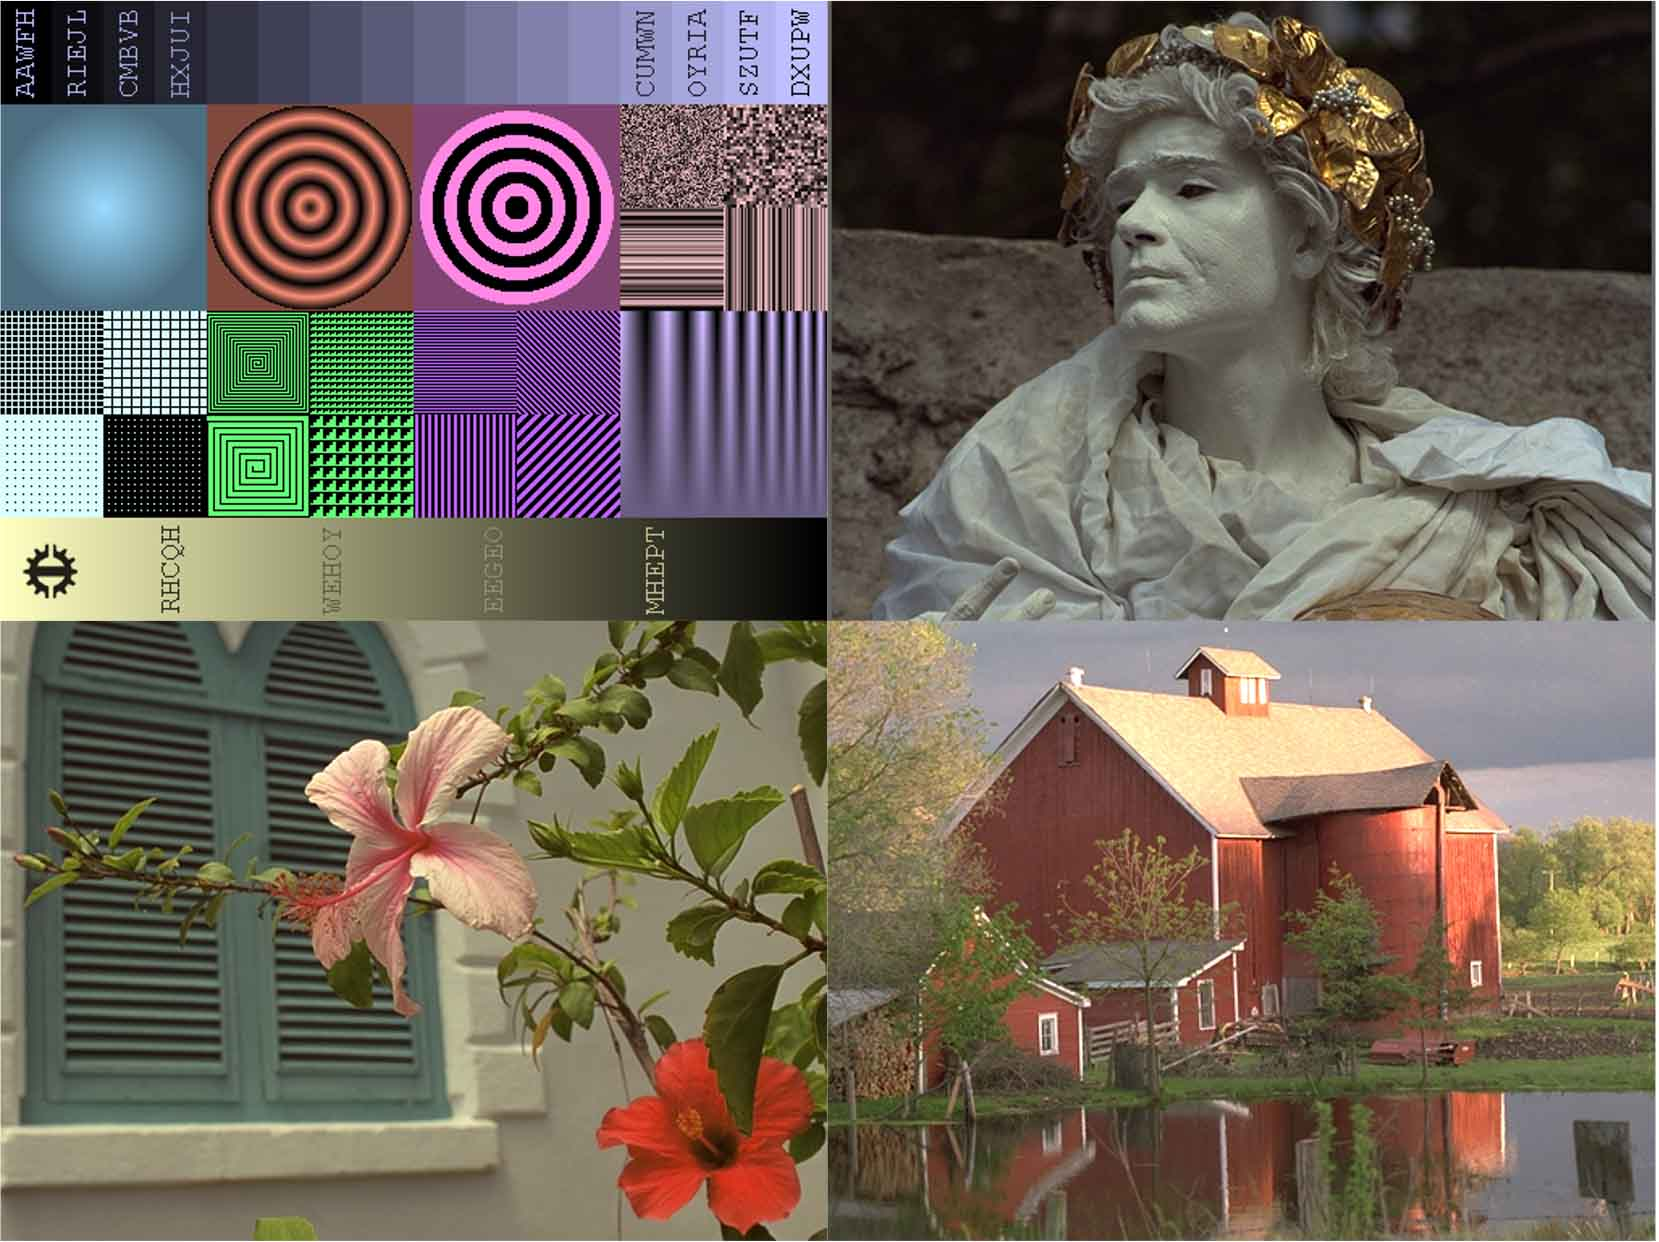
\includegraphics[width=2.8in]{fig/TID2013.jpg}
			\centerline{(c)}
		\end{minipage}
		\begin{minipage}[t]{.49\linewidth}
			\centering
			
\includegraphics[width=3in, height=2.1in]{fig/KADID.jpg}
			\centerline{(d)}
		\end{minipage}
		\caption{Natural images and a screen content image from the constructed databases. (a) LIVE Database~\citep{livedataset} (b) CSIQ Database~\citep{larson2010most} (c) TID2013 Database~\citep{ponomarenko2015image} (d) KADID-10k Database~\citep{kadid10k}.}
		\label{Databases}
	\end{figure}
	
	\subsection{Objective Image Quality Assessment}
	It is cumbersome, time-consuming, and costly to conduct subjective experiments and collect subjective opinions. On the other hand, objective IQA is much more practical, effective, efficient, and inexpensive. The objective IQA methods automatically assess the input image quality, playing an essential and fundamental role in various computer vision tasks, such as image enhancement, restoration, compression, synthesis, and generation~\citep{ding2021comparison, Kumar2022NR, Li2022SR, Mier2021, Li2021QA, isogawa2019better, zhang2019ranksrgan}. As mentioned above, its functionalities are automatic image quality assessment, performance evaluation of image processing systems, and model parameter optimization for image processing systems. Some objective image and video quality assessment methods have already been applied to image and video processing systems, such as the Netflix VMAF~\citep{li2016toward} and Google MUSIQ~\citep{ke2021musiq}. In specific, there are three kinds of objective IQA models categorized via the existence of pristine (reference) images,~\ie, the Full-reference (FR) IQA, Reduced-reference (RR) IQA, and No-reference (NR) IQA. The overall frameworks of the FR-IQA, RR-IQA, and NR-IQA are shown in~\reffig{IQA}.
	\begin{figure}[!ht]
		\centering
		\begin{minipage}[t]{\linewidth}
			\centering
			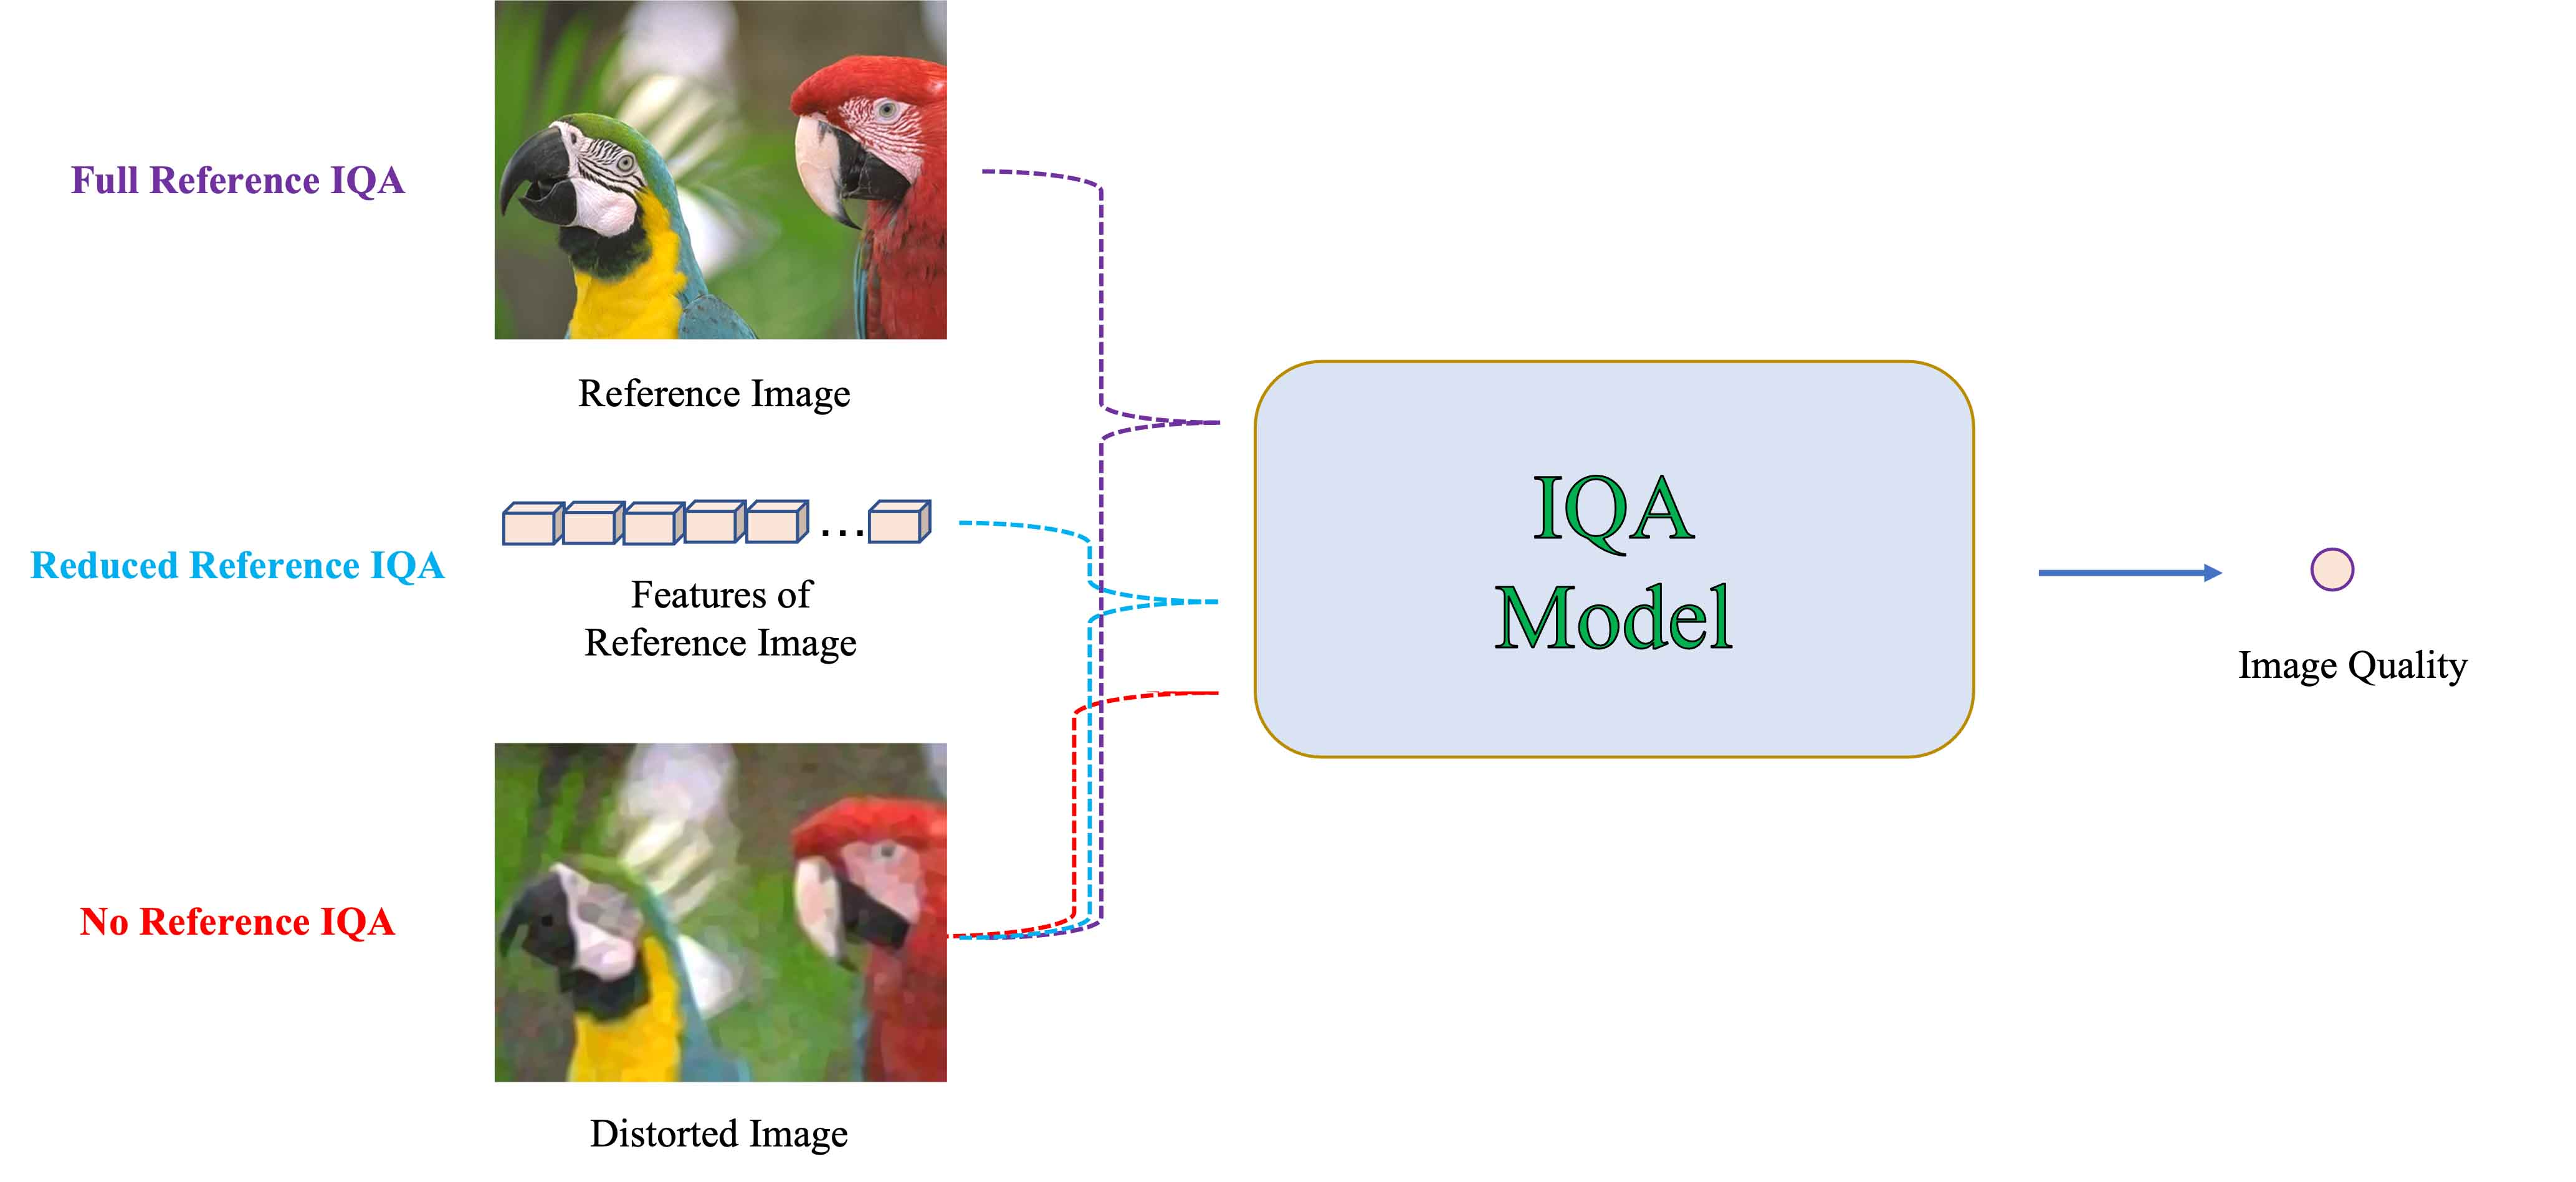
\includegraphics[width=6in]{fig/IQA.jpg}
		\end{minipage}
		\caption{FR-IQA, RR-IQA, and NR-IQA frameworks.}
		\label{IQA}
	\end{figure}
	
	The earliest objective IQA models can be dated back to the signal fidelity methods, such as the MSE and Peak Signal-to-noise Ratio (PSNR), which measure the fidelity difference between the pixel values of the reference image and the distorted image~\citep{wang2006modern}. The fidelity methods reflect the energy of the error signal, for instance, the sum of the squared error signal. In addition, such methods are mathematically easier to compute and optimize. However, due to some pre-defined assumptions, such as that the visual quality is unrelated to the pixel space, the visual quality is independent of the reference images when the error signals are unchanged, the visual quality only relies on error signals, and all pixels in the image are equally important, the MSE and PSNR methods are irrelevant to the subjective visual experience~\citep{wang2004image}. Thus, it inspires researchers to explore visually and perceptually relevant objective IQA methods.
	
	Over the past two decades, researchers have made substantial progress in IQA. History can be broadly separated apart by the emergence of deep learning technologies. Before the deep learning era, the research of objective FR-IQA is dramatically advanced by the Structural Similarity (SSIM)~\citep{wang2004image} and Visual Information Fidelity (VIF)~\citep{sheikh2006image}. For NR-IQA, the research has shifted from building models for a specific distortion,~\eg, image compression~\citep{zhu2014no, liu2018end}, JPEG~\citep{wang2002no}, JPEG2000~\citep{sheikh2005no}, blur~\citep{wang2003local}, and ringing artifacts~\citep{liu2009no}, to making general objective models in order to handle a variety of distortions. Based on the Natural Scene Statistics (NSS), the BRISQUE model is one of the representative works~\citep{mittal2012no}, which later motivated a series of NSS-based NR-IQA methods. Since 2014, a large amount of deep learning-based work has emerged in the study of IQA~\citep{yang2019comparative}, due to its robust learning and generalization capability.
	
	Because IQA tasks involve subjective perception and are challenging to model, recently, a growing number of research is based on data-driven learning-based methods. This method generally contains two modules,~\ie, feature extraction module and quality prediction module. During the training phase, after the handcrafted features are extracted from feature extraction module, quality prediction module can be trained with a loss function. During the testing phase, the quality score will be automatically predicted by encoding an image to the trained model. The deep learning-based model integrates two modules and will be jointly optimized, which performs superior to other data-driven models for IQA. The details of the FR-IQA, RR-IQA, and NR-IQA are described in the following.
	
	\subsection{Full-reference Image Quality Assessment}
	With the presence of reference images, the FR-IQA algorithms not only directly assess image quality~\citep{bosse2017deep}, but also optimize and evaluate image processing systems by developing an image fidelity metric as the loss function~\citep{ding2021comparison}. The inputs of the FR-IQA method are the distorted image with its corresponding reference image, and the output is the predicted quality score of the distorted image.
	
	\subsection{Reduced-reference Image Quality Assessment}
	%	\begin{figure}[!ht]
	%		\centering
	%		\begin{minipage}[t]{\linewidth}
	%			\centering
	%			\includegraphics[width=5.8in]{fig/RR-IQA.png}
	%		\end{minipage}
	%		\caption{General framework of the RR-IQA. \\Image by courtesy of Li~\etal\citep{li2009reduced}.}
	%		\label{RR-IQA}
	%	\end{figure}
	The RR-IQA algorithms maintain partial information from reference images, for example, a subset of features. Such methods are primarily employed for live television streaming services as they control the transmission quality on the fly~\citep{wang2011reduced}. The inputs of RR-IQA methods are the distorted image with partial information from its corresponding reference image, and the output is the predicted quality score of the distorted image.
	
	\subsection{No-reference/Blind Image Quality Assessment}
	Apart from FR and RR IQA, NR-IQA or blind IQA is highly desirable, practical, and essential in most real-life scenarios, where pristine images are hard to obtain~\citep{mittal2012no}. Since only the distorted image is encoded as input, NR-IQA methods can be applied to any scenarios. However, due to the lack of reference information, the research on NR-IQA is much more challenging. In practice, it evaluates visual quality when reference images are inaccessible, and estimates optimal parameters for image processing systems~\citep{mittal2012no, zhu2010automatic}. The output of NR-IQA models is the predicted quality score of the distorted image.

\section{Summary of Open Issues}
In this thesis, we concentrate on addressing two open issues in the field.

The first issue concerns the locality inductive bias of traditional local-modeling methods, which hinders the learning and generalization capability of IQA methods. The state-of-the-art visual quality assessment and perceptual optimization methods are primarily built upon traditional CNN, where strong inductive biases, such as locality, are inherent. Benefits abound in local processing, such as translation equivalence, translation invariance, and weight sharing. Nevertheless, the CNN filters extract features mainly from local neighborhoods. Thus, it is hard to catch the non-local features and long-range dependencies among pixels and regions from the image. Moreover, since the content in an image is multi-scale and space-variant, the CNN filters equally process it, which should be treated distinguishingly. Consequently, it lacks the capability to capture the unique content with its global context dependencies among objects and regions in the whole image. Furthermore, CNN can hardly model the geometric and relational causal dependencies. As such, suffered by the local priors to CNN, the non-local information is usually absent. The performance of local modeling methods may be improved by considering the non-local features and long-range dependencies.

The second issue concerns the poor generalization capability of current local-modeling methods. This problem leads to biased or even inaccurate guidance and evaluation results when IQA models are applied to evaluate image processing systems. For instance, the performance of image enhancement or restoration methods would be incorrect using a poor-generalized visual quality assessment model. Theoretically, deep learning methodology strongly assumes that the distributions of the validation and testing set should remain consistent with that of the training set. The testing, validation, and training data should draw from the same distribution and closely-aligned visual feature spaces. However, in practice, the captured images are highly diverse in terms of content and semantics, distortions, transmission mediums and methods, restoration, enhancement, resolution, environment, capturing device, and AI processing. In addition, since image space is enormous, the distributions of the validation and testing set may not abide by such an assumption. As a consequence, the generalization capability of IQA algorithms is of great essence in meeting the needs of real-life CV applications. From this perspective, the cross-database evaluation is one of the essential settings to verify the generalization capability of IQA methods. Thus, the poor cross-database performance of local modeling methods should be enhanced, making IQA models more applicable in real applications.

\section{Contributions of This Thesis}
In view of the above challenges and problems, in this thesis, we first analyze and discuss the non-local information and long-range dependencies on natural images. Then, a novel NR-IQA method based on the non-local features learned by Graph Neural Network (GNN) is proposed to explore the non-local information and long-range interactions in quality prediction. The main contributions of this thesis are outlined as follows:
\begin{itemize}
	\item We analyze the non-local modeling on natural images and summarize the significance of involving the non-local behavior in quality prediction and other CV tasks.
	\item Complementary to traditional local modeling methods, such as CNN, we propose a novel NR-IQA framework based on GNN. The non-local behavior of natural images is highlighted and learned in our proposed~\textbf{N}on-\textbf{L}ocal dependency~\textbf{Net}work (termed as~\textbf{NLNet}). The spatial attention module is introduced to integrate the information of long- and short-range communications among graph nodes of the entire image.
	\item Extensive experimental results reveal that the non-local modeling is complementary to traditional local methods. Both local and non-local features contribute to image quality assessment. In specific, CNN's local modeling features are critical and robust. Meanwhile, the non-local modeling is a supporting element that reinforces prediction power and boosts representation ability. The unilateral local features or non-local features will not truly be enough to evaluate perceptual quality. The combination of the two is superior for visual quality assessment.
	\item Experimental results of the individual distortion type indicate that the non-local modeling method manages to handle a wide variety of globally and uniformly distributed distortions with non-local recurrences. Meanwhile, it also maintains sensitivity to the local nonuniform-distributed distortions. In addition, it particularly holds a strong prediction power to assess the quality of noisy and compressed images. Lastly, the superior performance in the cross-dataset setting indicates the high generalization capability of our method, shedding light on the exploration of the generalized NR-IQA models.
\end{itemize}

\section{Outline of This Thesis}
This thesis consists of five chapters. An overview of this thesis is as follows:

In Chapter~\ref{chap:introduction}, we introduce the background, significance, and functionalities of visual quality assessment, subjective IQA, and objective IQA. Then, some subjective methods are described to construct an IQA database, as defined in the Recommendation ITU-R BT.500-14. Next, the details of FR-IQA, RR-IQA, and NR-IQA are presented. Further, two open issues and the contributions of this thesis are summarized. Finally, we outline the organization of this thesis.

In Chapter~\ref{chap:related_work}, we review and summarize some related works of the objective IQA,~\ie, FR-IQA, RR-IQA, and NR-IQA. In specific, we first introduce the development of FR-IQA, from signal fidelity and error sensitivity to the SSIM, VIF, and data-driven learning-based methods. Then, feature extractions of RR-IQA methods in the spatial and transform domains are reviewed, respectively. Finally, NR-IQA models based on Human Visual System (HVS), NSS, and codebook are separately presented.

In Chapter~\ref{chap:chapter3}, we analyze and discuss the local and non-local modeling for natural images. Firstly, the local modeling analysis of natural images and the advantages of the local modeling methods are presented. Then, we present the non-local modeling analysis of natural images from the viewpoints of non-local statistics, non-local dependency and relational modeling, and effective image-specific prior. As evident from demonstrations, we summarize the significance of the non-local modeling for CV tasks.

In Chapter~\ref{chap:chapter4}, we propose an NR-IQA method based on the non-local features learned by GNN. We first adopt superpixel segmentation for graph nodes construction. Subsequently, a spatial attention module is proposed to integrate long- and short-range dependencies among the nodes of the whole image. The learned non-local features are finally combined with the local features extracted by the pre-trained CNN, achieving superior performance to features utilized individually.

Finally, we summarize the work of this thesis and look forward to further research directions in Chapter~\ref{chap:conclusion}.
